\newpage
\subsection{Programmierschnittstellen}
\label{sec:Inbetriebnahme_Programmierschnittstellen}

Die Programmierschnittstellen werden jeweils mithilfe eines USB-UART-Controller gesteuert. Im Folgenden wird die Inbetriebnahme dieser Schnittstelle für den Mikrocontroller und das Bluetooth-/Wifimodul beschrieben. Beide werden über eine USB-B-Buchse realisiert.

Für die Inbetriebnahme der USB-B-Schnittstelle wurde vorerst geprüft, ob der USB-UART-Converter über die USB-Buchse und Kabel vom Computer erkannt wird. Danach wurde geprüft, wie der Handshake beim Programmieren der Komponenten funktioniert. Die Inbetriebnahme der Programmierung geschieht parallel zur Inbetriebnahme der Programmierschnittstelle, da die Programme zum Schreiben, Kompilieren und Hochladen des Codes schon vor dem Prüfen der USB-B-Schnittstelle installiert sein müssen. Da ein erfolgreicher Handshake als Voraussetzung gilt, dass überhaupt ein Programm hochgeladen werden kann, wurde entschieden, dass der Handshake zur Programmierschnittstelle gehört. Die Programmierung der Targets (Mikrocontroller und WiFi-Modul) wird in den Kapitel \ref{subsubsec:Inbetriebnahme_ESP} und Kapitel \ref{subsec:Inbetriebnahme_Mikrocontroller} beschrieben. Um den Handshake zu kontrollieren sind die in Abbildung \ref{fig:USB_B_Print} eingekreisten Punkte interessant:


\begin{figure}[h!]
\center
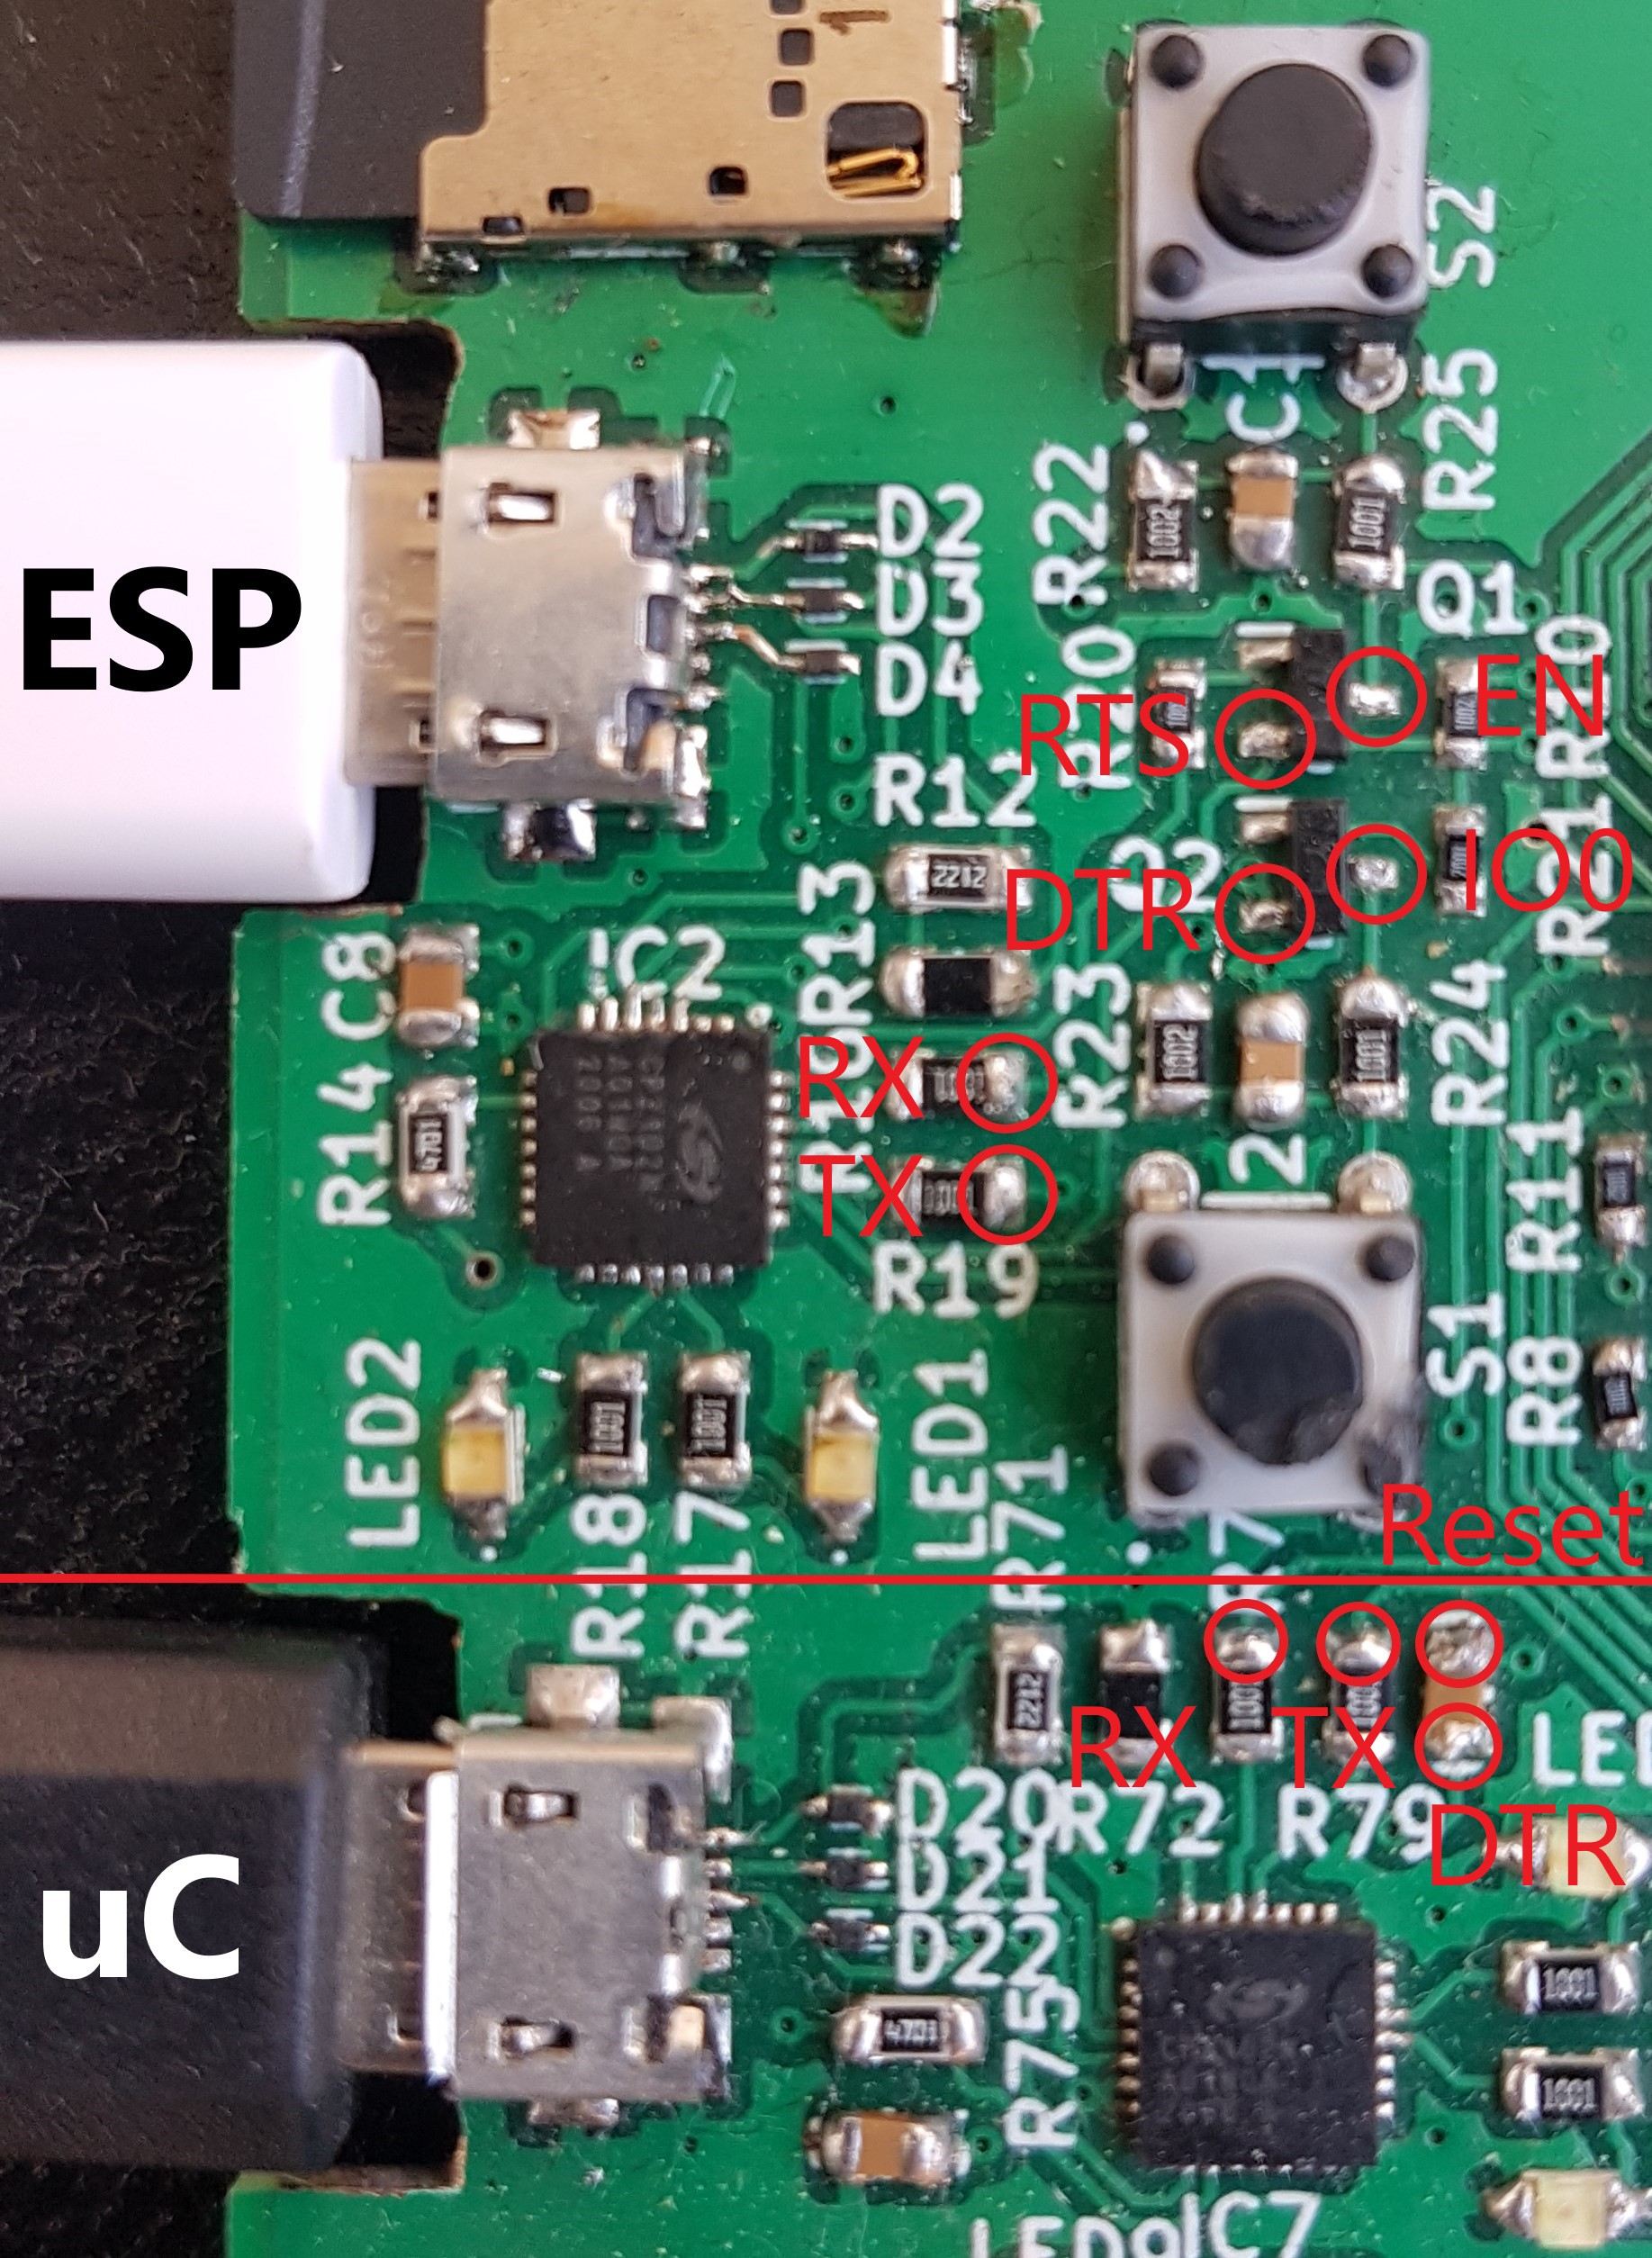
\includegraphics[width = 0.58\textwidth]{graphics/USB_B_Print}
\caption{Ausschnitt aus Platine (USB-Scnittstellen) mit eingekreisten Messpunkten.}
\label{fig:USB_B_Print}
\end{figure}

\todo{Kim bitte bessere Bildmarkierungen einfügen, welche besser sichtbar sind. Danke}

Für die Inbetriebnahme der Programmierschnittstellen wurde mit der entsprechenden Programmierumgebung ein HEX-File mit dem darin enthaltenen Code übertragen und die in Abbildung \ref{fig:USB_B_Print} markierten Punkte gemessen.
\newpage
Vorgehen:

\begin{enumerate}
\item Platine mit Spannung versorgen und Computer mit zwei USB-Kabeln an die USB-B-Buchsen anschliessen.\\
\textcolor{blue}{Systemeinstellungen\textrightarrow Geräte-Manager}\\
Dort sind die Devices sichtbar unter dem Name: \textit{Silicon Labs CP210x USB to UART Bridge}. Die Verifizierung ist im Anhang Kapitel \ref{Appendix:Geraete_Manager} zu finden.\newline
\item Überprüfen der Handshakes, welche definiert sind in den Tools zum Hochladen der Software.\\

\begin{enumerate}
\item Mikrocontroller\\

Um zu evaluieren, wie der Handshake durchgeführt wird, wurde beim Hochladen eines Programms an den markierten Punkten auf der unteren Seite in Abbildung \ref{fig:USB_B_Print} gemessen.\\

Im Anhang Kapitel \ref{Appendix:Handshake_uC} ist der Handshake und die Übertragung der ersten Bytes zu sehen. Der Handshake wird in einer weiteren Abbildung des selben Kapitels genauer aufgezeigt. Darin ist erkennbar, dass sobald die DTR-Leitung auf GND gezogen wird und die Spannung über dem Reset-Pin aufgrund des Kondensators zwischen DTR und Reset nur kurzzeitig auf 0V fällt. Dies reicht jedoch aus, dass der Mikrocontroller in den Boot-Modus fällt. Nach ca. 50ms beginnt die Datenübertragung vom Computer in den Flash-Speicher des Mikrocontrollers.\\

\item WiFi-Modul\\

Um zu evaluieren, wie der Handshake durchgeführt wird, wurde beim Hochladen eines Programms an den markierten Punkten auf der oberen Seite in Abbildung \ref{fig:USB_B_Print} gemessen.\\

Im Anhang Kapitel \ref{Appendix:Handshake_ESP_Messung} wurden die ersten 100ms des Hochladen eines Programms auf das WiFi-Modul gemessen. Gesucht wird nach einem gleichzeitigen Flankenwechsel der RTS-Leitung von 0 auf 1 und der DTR-Leitung von 1 nach 0. Eine weitere Abbildung im selben Kapitel zeigt eine genauere Aufnahme zum Zeitpunkt des Flankenwechsels.

Was bei genauerem Betrachten der Messungen auffällt: Entgegen der Erwartung ist der Flankenwechsel der beiden Leitungen leicht verzögert (um ca. 80 \textmu s). Auch das Signal des EN-Pins erreicht wesentlich schneller einen HIGH-Zustand als erwartet. Denn gemäss der Theorie müssen die Pins EN und IO0 zum gleichen Zeitpunkt auf LOW sein, um in den Download-Boot-Modus zu kommen, und trotz der Abweichung der Praxis zur Theorie funktioniert die Übertragung des Codes. Eine kleine Erläuterung zu dieser Abweichung ist im Anhang Kapitel \ref{Appendix:Handshake_ESP_Messung} zu finden. Schlussfolgerung davon ist, dass die Strapping-Pins wahrscheinlich erst nach einer gewissen Zeit gelesen werden und so die angelegten Zustände erst zu einem späteren Zeitpunkt von Bedeutung sind.

\end{enumerate}

\end{enumerate}


Über LED's kann angezeigt werden, ob eine Übertragung zwischen den Komponenten stattfindet. Pro Schnittstelle jeweils ein LED für RX und ein LED für TX. Diese funktionieren leider nicht. Dazu müsste wahrscheinlich ein Register des USB-UART-Converters gesetzt werden oder ggf. die Vorwiderstände der LED's angepasst werden.